\section{Quantile Regression based time series model} \label{sec:qr1}

Let the $\alpha$-conditional quantile function of $Y$ for a given value $x$ of the $d$-dimensional random variable $X$, i.e., $Q_{Y|X}:[0,1] \times \mathbb{R}^d \rightarrow \mathbb{R}$, can be defined as %(in short, from now on, $Q_{Y|X}(\cdot, \cdot)$)
	\begin{equation}
	Q_{Y|X}(\alpha,x) = F_{Y|X=x}^{-1}(\alpha) = \inf\{y: F_{Y|X=x}(y) \geq \alpha\}.
	\label{eq:quantile-function}
	\end{equation}
The Conditional Quantile Function $Q$ is the inverse of the Distribution Function $F$, and represents the smallest value $y$ for which the distribution function is greater than a given probability $\alpha$.

Let $\rho$ be the check function 
	\begin{equation}\label{eq:check-function}
	\rho_{\alpha}(x)=\begin{cases}
	\alpha x & \text{if }x\geq0\\
	(1-\alpha)x & \text{if }x<0
	\end{cases}.
	\end{equation}
The quantile function for a given finite sample $\{y_t,x_t \}_{t \in T}$, where $T$  is the set of time indexes, and a given probability $\alpha$ is the solution of minimizing the loss function $L_\alpha(\cdot)$:
	\begin{IEEEeqnarray}{C}
	\hat{Q}_{Y|X}(\alpha,\cdot)\quad\in\quad  \underset{q\in\mathcal{Q}}{\text{arg min}}\, L_\alpha(q) = \sum_{t\in T}\rho_{\alpha}(y_{t}-q(x_t)).\label{eq:optim-lqr1} 
	\end{IEEEeqnarray}
For Inference on Quantile Regression and finite sample properties, see the Chapter 3 on \cite{koenker2005quantile}.
The $\alpha$-quantile function $q(\cdot)$ belongs to a function space $\mathcal{Q}$. We might have different assumptions for space $\mathcal{Q}$, depending on the type of function we want to find 
for $q$. A few properties, however, must be achieved by our choice of space, such as being continuous and having limited first derivative. In this work, we consider the following two cases: 
\begin{enumerate}
	\item $\mathcal{Q}$ is a linear function space such that
		$q_\alpha(x_t) = \beta_0 + \beta^T x_t;$ 
	\item $\mathcal{Q}$ is a space of continuous functions with limited first and second derivatives.
\end{enumerate}

% Let the finite discretization of the interval $[0,1]$ be composed of a sequence of probabilities $0 < \alpha_1 < \alpha_2 < \dots < \alpha_{|J|} < 1$ and denote as $A$ the set $A = \{ \alpha_j \mid j \in J \}$, where $J$ is an index set for the probabilities $\alpha$.
% In the next subsections\todo{se fala assim?}, we present in more details how to use the two aforementioned hypothesis for $\mathcal{Q}$ and estimate a sequence of quantiles $\{ q_{\alpha_j} \}_{j\in J}$. 


\subsection{Linear Model}

The linear model presumes that the $\alpha$-quantile function is a linear function of its regressors:
$$q_{\alpha}(x_t) = \beta_{0} + \beta^T x_t.$$   
When dealing with many candidates of covariates, one has to deal with the problem of selecting the relevant ones out of a set of candidates which improve model fit. In practice, it means that some coefficients from the vector $\beta = [ \beta_{1 } \cdots \beta_{p} ]$ might assume zero value.
There are many ways of selecting a subset of variables among the available options.
A classical approach for this problem is the Stepwise algorithm \cite{efroymson1960multiple}, \cite{hocking_selection_1967}, \cite{tibshirani1996regression}, which includes variables in sequence. 

A popular way of variable selection which fits on a linear programming context are the LASSO/AdaLASSO techniques, which consists in penalizing the $\ell_1$-norm. Besides shrinking coefficients towards to zero, it has also the capability of effectively pushing coefficients to zero (an effect that ridge regression cannot achieve \cite{tibshirani1996regression}). The usage of LASSO and AdaLASSO in QR context is the topic of study in \cite{li_l1-norm_2008,ciuperca_adaptive_2016,belloni_l1-penalized_2009,zou_regularized_2008,jiang_interquantile_2014}.
We refer to the reader the work from \cite{belloni_l1-penalized_2009}, where it is possible to find specific properties and convergence rates when using the LASSO to perform model selection in a quantile regression framework. 

Regarding the penalization parameter $\lambda$, which dictates the shrinkage magnitude of the linear coefficients, the level of parsimony of the model can be defined by the user through such quantity. This is due to the fact that higher values of $\lambda$ means less variables selected to be non-zero. 

The single $\alpha$-quantile AdaLASSO is estimated by the following optimization problem:
\begin{IEEEeqnarray}{c}
\underset{\beta_{0},\beta}{\text{min}} \sum_{t \in T} \rho_\alpha(y_t - (\beta_0 + \sum_{p \in P} \beta_p x_{tp})) +\lambda \sum_{p \in P} w_p | \beta_p |.\label{eq:l1-qar-optim} 
\end{IEEEeqnarray}
What differs the AdaLASSO from the LASSO is the inclusion of the term $w_p$. Suppose the model (\ref{eq:l1-qar-optim}) is estimated with all $w_{p}=1$, the output of the optimization problem are coefficients of LASSO  $\beta^{L}_{p}$. The AdaLASSO coefficients $\beta^{AL}_{p}$ are obtained when solving the same optimization problem while letting $w_{p}=1/|\beta^{L}_{p}|$. 
% What differs the AdaLASSO from the LASSO is the inclusion of the term $w_p$. Suppose the model (\ref{eq:l1-qar-optim}) is estimated with all $w_{pj}=1$, the output of the optimization problem are coefficients of LASSO  $\beta^{L}_{pj}$. The AdaLASSO coefficients $\beta^{AL}_{pj}$ are obtained when solving the same optimization problem while letting $w_{pj}=1/|\beta^{L}_{pj}|$. % para voltar o 'j'






\subsection{Nonparametric Quantile Regression}
\label{sec:npqar}

Fitting a linear estimator for the QR is less attractive when nonlinearity is present in the quantile functions. In Figure \ref{fig:nonlinear}, a nonlinear relationship between variables $x$ and $y$ is presented, where $y = x^2 + error$. When using a linear estimator for this type of relation, this estimator underestimates the quantile for a chunk of data while overestimating for the other chunk. In cases such as this, a nonlinear estimator for the quantiles produces better results.
\begin{figure}[t]
	\begin{center}
	  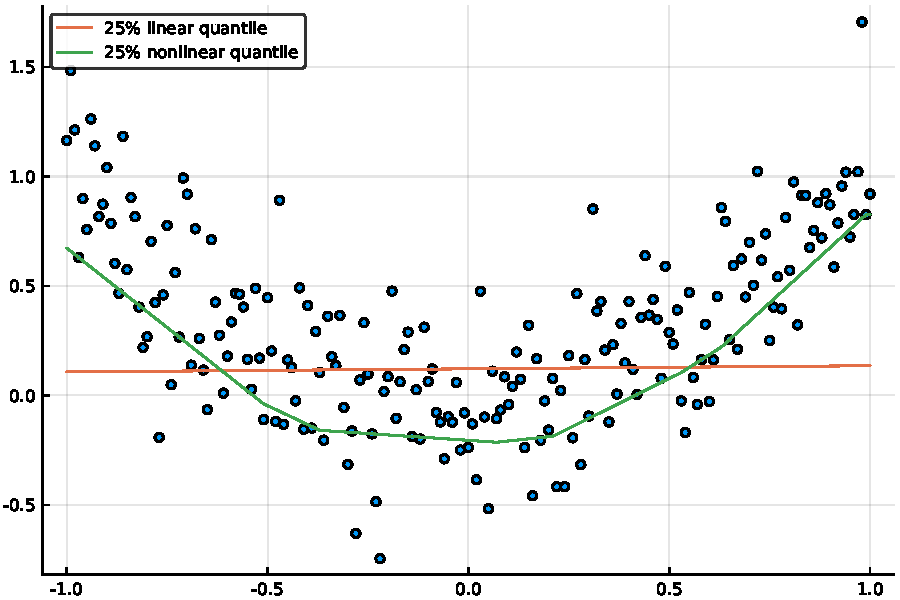
\includegraphics[width=0.7\textwidth]{Images/nonlinear}
	\end{center}
	\caption{Calculating the 25\% quantile with both methodologies when there is a nonlinear relationship between $x$ and $y$. While the linear estimator fails to estimate the conditional quantile, the nonlinear estimator is able to capture the quadratic dependency.}
	\label{fig:nonlinear}
\end{figure}
Comparing both quantile estimator, it is clear that the nonparametric is capable of capturing the nonlinearity on the relationship, while the linear model can only capture linear relationships.

A nonlinear estimator is built by allowing the quantile function $q(\cdot)$ to freely adjust to the data. The only required aspects for $q$ are being continuous and having limited first and second derivatives.
In order to acomplish this, we introduce a Nonparametric Quantile Autoregressive model with a $\ell_{1}$-penalty term on both the first and second derivatives, represented by their discrete aproximation $D^1 q_t$ and $D^2 q_t$ on equations (\ref{eq:d1qt}) and (\ref{eq:d2qt}), respectively, presented below:
\begin{equation}
  D^{1}_{tj}=\frac{q_{t+1}-q_{tj}}{x_{t+1}-x_{t}},\label{eq:d1qt}
\end{equation}
\begin{equation}
D_{x_{t}}^{2}q_{t}=\frac{\left(\frac{q_{t+1}-q_{t}}{x_{t+1}-x_{t}}\right)-\left(\frac{q_{t}-q_{t-1}}{x_{t}-x_{t-1}}\right)}{x_{t+1}- x_{t-1}}.\label{eq:d2qt}
\end{equation}


% To prevent overfitting and smoothen our predictor, we include a penalty on its roughness by including the $\ell_1$ norm of its second derivative. For more information on the $\ell_1$ norm acting as a filter, one can refer to \cite{kim2009ell_1}.

% This time, as opposed to when employing linear models, we don't suppose any functional form for $q_\alpha(x_t)$. This forces us to build each $q_\alpha$ differently: instead of finding a set of parameters that fully defines the function, we find a value for $q_\alpha(x_t)$ at each instant $t$. On the optimization problem, we will find optimal values for a variable $q_{tj} \in \mathbb{R}$, each consisting of a single point. The sequence  $\{ q^*_{\alpha t} \}_{\alpha \in A} $ will provide a discretization for the quantile function $\hat{q}_\alpha(x_t)$, which can be found by interpolating these points.

% notação estatística de ordem. com x^(0)


Let $\{\tilde{y}_t \}_{t=1}^n$ be the sequence of observations in time $t$ and let $\tilde{x}_t$ be the $p-$lagged time series of $\tilde{y}_t$, such that $\tilde{x}_t = L^p(\tilde{y}_t)$, where $L$ is the lag operator. Matching each observation $\tilde{y}_t$ with its $p-$lagged correspondent $\tilde{x}_t$ produces $n-p$ pairs $\{(\tilde{y}_t,\tilde{x}_t)\}_{t=p+1}^n$ (note that the first $p$ observations of $y_t$ must be discarded). When the sequence of observations of $x$ are reorder in such a way that they are in growing order
$$\tilde{x}^{(p+1)} \leq \tilde{x}^{(p+2)} \leq \dots \leq \tilde{x}^{(n)},$$ 
the new sequences can be defined $\{x_i\}_{i=1}^{n-p} = \{\tilde{x}^{(t)} \}_{t=p+1}^{n}$ and $\{y_i\}_{i=1}^{n-p} = \{\tilde{y}^{(t)} \}_{t=p+1}^{n}$, where $T' = \{2,\dots, n-p-1\}$. 
% The optimization model to estimate the nonparametric quantile is as follows:
% \begin{equation}
% \begin{split}
% \hat{q}_{\alpha_j}(x_t) =\underset{q_{tj}}{\arg\min}\sum_{t\in T'} \rho_{\alpha_j} \left( y - q_{tj} \right) \\ +\lambda_1  \sum_{t\in T'}|D_{x_t}^{1}q_{tj}| +\lambda_2  \sum_{t\in T'}|D_{x_t}^{2}q_{tj}|,
% \end{split}
% \end{equation}
% where $D^1 q_t$ and $D^2 q_t$ are the first and second derivatives of the $q_\alpha(x_t)$ function, calculated as follows:
% \begin{equation*}
% D_{x_{t}}^{2}q_{tj}=\frac{\left(\frac{q_{\alpha t+1}-q_{tj}}{x_{t+1}-x_{t}}\right)-\left(\frac{q_{tj}-q_{\alpha t-1}}{x_{t}-x_{t-1}}\right)}{x_{t+1}- x_{t-1}},
% \end{equation*}
The optimization model to estimate the $\alpha$-quantile nonparametrically is as follows:
\begin{equation}
\begin{split}
\hat{q}_{\alpha}(x_t) =\underset{q_{t}}{\arg\min}\sum_{t\in T'} \rho_{\alpha} \left( y - q_{t} \right) \\ +\lambda_1  \sum_{t\in T'}|D_{x_t}^{1}q_{t}| +\lambda_2  \sum_{t\in T'}|D_{x_t}^{2}q_{t}|.
\end{split}
\end{equation}
The purpose of the filters, then, is to control the amount of variation for the estimator $q_\alpha(x_t)$. When no penalty is employed, the estimated quantile always match the observations $q_{tj} = y_t$, for any given $\alpha$. On the other hand, when $\lambda_2 \rightarrow \infty$, the estimator approaches the linear quantile regression. 

%The first part on the objective function is the usual Loss function for $\{q_{t\alpha}\}_{\alpha \in A}$. The second part are the $\ell_1$-filters. The purpose of the filters is to control the amount of variation for the estimator $q_\alpha(x_t)$. When no penalty is employed we would always get $q_{tj} = y_t$, for any given $\alpha$. On the other hand, when $\lambda_2 \rightarrow \infty$, our estimator approaches the linear quantile regression. 





